\section{Lecture 33 — Geometric Constructions I}

\begin{definition}[straightedge, compass]
	A \textbf{straightedge} is an \textit{unmarked} tool used to draw lines between points. A \textbf{compass} is a tool used to draw circles centered at a fixed point with a fixed radius. Our compass is ``collapsible'' i.e. lifting the compass resets the separation of the legs.

	A \textbf{straightedge and compass construction} is any drawing in the plane that can be made using a straightedge and a compass, following the following rules.
\end{definition}

\begin{enumerate}[label={\bfseries\sffamily\color{main}\arabic*.}]
	\item Given two points, we can construct a line between them.
	\begin{center}
	\begin{tikzpicture}
		\draw (-1.5,0) -- (1.5,0);
		\node[circle,fill,main,scale=0.5] at (-1,0) {};
		\node[circle,fill,main,scale=0.5] at (1,0) {};
	\end{tikzpicture}
	\end{center}
	\item Given two points, we can construct a circle centered at a point with the other on the circumference.
	\begin{center}
	\begin{tikzpicture}
		\draw (0,0) circle (1);
		\node[circle,fill,main,scale=0.5] at (0,0) {};
		\node[circle,fill,main,scale=0.5] at (60:1) {};
	\end{tikzpicture}
	\end{center}
	\item Intersecting two lines constructs a point.
	\begin{center}
	\begin{tikzpicture}
		\draw (-1,-0.5) -- (1,0.5);
		\draw (-1,0.5) -- (1,-0.5);
		\node[circle,fill,main,scale=0.5] at (0,0) {};
	\end{tikzpicture}
	\end{center}
	\item Intersecting a line and a circle constructs one or two points.
	\begin{center}
	\begin{tikzpicture}
		\begin{scope}
		\draw (0,0) circle (1);
		\draw (190:1.25) -- (10:1.25);
		\node[circle,fill,main,scale=0.5] at (190:1) {};
		\node[circle,fill,main,scale=0.5] at (10:1) {};
		\end{scope}
		\begin{scope}[shift={(3,0)}]
		\draw (0,0) circle (1);
		\draw (1,-1) -- (1,1);
		\node[circle,fill,main,scale=0.5] at (1,0) {};
		\end{scope}
	\end{tikzpicture}
	\end{center}
	\item Intersecting two circles constructs one or two points.
	\begin{center}
	\begin{tikzpicture}
		\begin{scope}
		\draw (0.5,0) circle (1);
		\draw (-0.5,0) circle (1);
		\node[circle,fill,main,scale=0.5] at (0,{sqrt(3)/2}) {};
		\node[circle,fill,main,scale=0.5] at (0,{-sqrt(3)/2}) {};
		\end{scope}
		\begin{scope}[shift={(4,0)}]
		\draw (1,0) circle (1);
		\draw (-1,0) circle (1);
		\node[circle,fill,main,scale=0.5] at (0,0) {};
		\end{scope}
	\end{tikzpicture}
	\end{center}
\end{enumerate}

The following question naturally arises:

\begin{rmkbox}
	Using the above rules, what can we make?
\end{rmkbox}

\begin{example}
	We can construct the midpoint between any two points.
	\begin{proof}
		Given two points $P_1$ and $P_2$, follow these steps:
		\begin{enumerate}[label={\bfseries\sffamily\color{main}(\arabic*)}]
			\item Draw a line $L_1$ between $P_1$ and $P_2$.
			\item Draw a circle $C_1$ with center $P_1$ and circumference point $P_2$.
			\item Draw a circle $C_2$ with center $P_2$ and circumference point $P_1$.
			\item Label the intersections of these circles $Q_1$ and $Q_2$.
			\item Draw a line $L_2$ passing through $Q_1$ and $Q_2$.
			\item The intersection $M$ of $L_1$ and $L_2$ is the midpoint of $P_1$ and $P_2$
		\end{enumerate}

		\begin{center}
		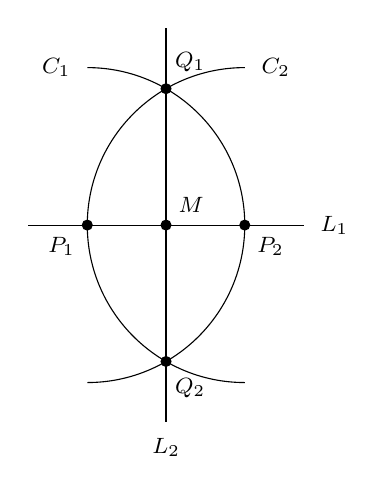
\begin{tikzpicture}
			\footnotesize
			\draw (-1.75,0) -- (1.75,0) node[label={right:$L_1$}] {};
			%\draw (-1,0) circle (2);
			\draw (-1,-2) arc (-90:90:2) node[label={left:$C_1$}] {};
			\draw (1,-2) arc (270:90:2) node[label={right:$C_2$}] {};
			\node[circle,fill,scale=0.5,label={below left:$P_1$}] at (-1,0) {};
			\node[circle,fill,scale=0.5,label={below right:$P_2$}] at (1,0) {};

			\node[circle,outer sep=0pt,fill,scale=0.5,label={[label distance=1pt]85:$Q_1$}] at (0,{sqrt(3)}) {};
			\node[circle,outer sep=0pt,fill,scale=0.5,label={[label distance=1pt]-85:$Q_2$}] at (0,{-sqrt(3)}) {};

			\draw (0,2.5) -- (0,-2.5) node[label={below:$L_2$}] {};

			\node[circle,fill,scale=0.5,label={above right:$M$}] at (0,0) {};
		\end{tikzpicture}
		\end{center}
	\end{proof}
\end{example}

\begin{example}
	There are other constructions that can be made using the outlined rules:
	\begin{itemize}
		\item The previous example shows that we can construct a perpendicular bisector.
		\item Given a line segment $\overline{AB}$, we can create a square with side length $AB$.
		\item Given a line $L$ and a point $P$ off of $L$, we can create a line $L'$ passing through $P$ and parallel to $L$.
		\item Given a rectangle with area $A$, we can construct a square with area $A$.
		\item Given an angle $\theta$, we can construct the angle $\theta/2$. That is, any angle can be bisected.
	\end{itemize}
\end{example}

Asking what \textit{can} be constructed gave rise to some classical problems:
\begin{rmkbox}
	\begin{enumerate}
		\item Trisecting an arbitrary angle.
		\item Squaring the circle.
		\item Doubling the cube.
	\end{enumerate}
\end{rmkbox}

Neither of these constructions are possible! We need field theory to prove this. Constructions (a) and (c) were proved not possible by Wentzel in 1837 and (b) follows from Lindemann's 1882 proof that $\pi$ is transcendental.

The proofs will be discussed in more detail next lecture. First, we need to set up some vocabulary and prove some intermediate results.

\begin{definition}[constructible number]
	A real number $\alpha$ is \textbf{constructible} if a line segment of length $|\alpha|$ can be constructed in the plane in a finite number of steps using only a straightedge and compass
\end{definition}

\begin{example}
	Every element of $\mathbb Z$ is constructible.

	\begin{center}
	\begin{tikzpicture}
		\footnotesize

		\draw[->] (-3.5,0) -- (5.5,0);
		\foreach \i in {-2,-1,...,4}{
		\draw[main,opacity=0.5] (\i,0) circle (1);
		}
		\foreach \i in {-2,-1,...,4}{
		\draw[|-] (\i,0) node[below] {\i} -- ({\i+1},0);
		}
		\draw (-3,0) -- (5,0);
	\end{tikzpicture}
	\end{center}

	Note that $\frac 12$ can be constructed by taking a midpoint.
\end{example}

\begin{theorem}
	The set of all constructible numbers $F$ is a subfield of $\mathbb R$.
\end{theorem}

\begin{proof}
	Given $\alpha,\beta\in F$, we need to show $\alpha\pm\beta\in F$, $\alpha\beta\in F$ and $\frac{\alpha}{\beta}\in F$.

	Without loss of generality, suppose $\alpha>\beta$.
	\begin{center}
	\begin{tikzpicture}
		\footnotesize
		\draw[|-|] (0,0) -- node[midway,above] {$\alpha$} (3,0);
		\draw[|-|] (4,0) -- node[midway,above] {$\beta$} ++(2,0);
	\end{tikzpicture}
	\end{center}

	The segments can be joined together to form $\alpha+\beta$.

	\begin{center}
	\begin{tikzpicture}
		\footnotesize
		\draw[|-|] (0,0) -- node[midway,above] {$\alpha$} (3,0);
		\draw[|-|] (3,0) -- node[midway,above] {$\beta$} ++(2,0);
		\draw[decorate,decoration={brace,mirror},main] (0,-0.25) -- node[midway,below] {$\alpha+\beta$} (5,-0.25);
	\end{tikzpicture}
	\end{center}

	Similarly, the segments can be superimposed to form $\alpha-\beta$.

	\begin{center}
	\begin{tikzpicture}
		\footnotesize
		\draw[|-|] (0,0) -- node[midway,above=12pt] {$\alpha$} (3,0);
		\draw[|-|] (1,0) -- node[midway,above] {$\beta$} ++(2,0);
		\draw[decorate,decoration={brace,mirror},main] (0,-0.25) -- node[midway,below] {$\alpha-\beta$} (1,-0.25);
	\end{tikzpicture}
	\end{center}

	To construct $\alpha\beta$, consider the case where $\beta>1$ and form a triangle with sides of length 1 and $\alpha$, where the sides of length $1$ and $\alpha$ join at the point $P$. Call the other side $L$. Extend the side of length 1 to $\beta$ and call the endpoint $R$. Draw a line $M$ through $R$ parallel to $L$ and intersect it with an extension of the segment of length $\alpha$. Call the intersection $Q$. Then the length $PQ$ is $\alpha\beta$.

	\begin{center}
	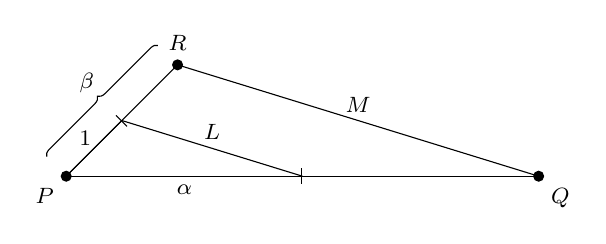
\begin{tikzpicture}
		\footnotesize
		\draw[-|] (0,0) -- node[midway,below] {$\alpha$} (3,0);
		\draw[-|] (0,0) -- node[midway,above left=-2pt] {1} (45:1);
		\draw (45:1) -- node[midway,above] {$L$} (3,0);
		\draw (0,0) -- (45:2);
		\draw[decorate,decoration={brace},shift={(135:0.35)}] (0,0) -- node[midway,above left] {$\beta$} (45:2);
		\draw (45:2) -- node[midway,above] {$M$} (6,0);
		\draw (0,0) -- (6,0);

		\node[fill,circle,scale=0.5,label={below left:$P$}] at (0,0) {};
		\node[fill,circle,scale=0.5,label={below right:$Q$}] at (6,0) {};
		\node[fill,circle,scale=0.5,label={above:$R$}] at (45:2) {};
	\end{tikzpicture}
	\end{center}

	This works by similar triangles: $\frac 1\alpha=\frac{\beta}{PQ}\Rightarrow PQ=\alpha\beta$.

	The construction of $\frac{\alpha}{\beta}$ is left as an exercise.
\end{proof}